\documentclass[12pt, a4paper]{article}
\usepackage[utf8]{inputenc}
\usepackage{graphicx}
\usepackage{gensymb}
\usepackage{amsmath}
\usepackage{float}
%\usepackage[figurename=Graf]{caption}
\usepackage{subcaption}
\usepackage{caption}


\title{Title}
\author{Miha Pompe}
\date{January 2022}

\begin{document}
\begin{titlepage}
	\centering
 	
\includegraphics[width=0.45\textwidth]{logo_fmf_uni-lj_sl_veliki.png}\par\vspace{1cm}

	\vspace{1cm}

	\vspace{1.5cm}
	{\huge\bfseries Gelarkin method \par}
	\vspace{2cm}
	{\Large Miha Pompe 28191072\par}
	\vfill

	\vfill

% Bottom of the page
	{\large January 2022\par}
\end{titlepage}
% \maketitle
\thispagestyle{empty}
\clearpage
\pagenumbering{arabic}
\newpage


\section{Introduction}
To describe one-dimensional laminar flow of a viscous and non compressible fluid through a long pipe that is flowing due to a pressure gradient $p'$ we use Navier-Stokes equations that in this case simplify into Poisson equation
\begin{equation*}
  \nabla^2 v = -\frac{p'}{\eta}
\end{equation*}
where $v$ is the parallel component of velocity, that is dependent only on coordinates of the cross section. $\eta$ is the viscosity of the fluid. We want to solve the equation on the inside of the pipe, as the velocity at the boundary is equal to zero. The flow through the pipe obeys the Poiseuille's law
\begin{equation*}
  \Phi = \int_S vdS = C\frac{p'S^2}{8\pi\eta}
\end{equation*}
where $C$ is a coefficient that is dependent only on the shape of the pipe. In this exercise we will try to determine this coefficient for a half circular pipe of radius $R$. Let's introduce some new variables $\xi = r/R$ and $u = v\eta/p'R^2$. Our problem is now:
\begin{equation*}
  \Delta u(\xi,\phi) = -1 \>,\qquad
  u(\xi=1,\phi)=u(\xi,0)=u(\xi,\phi=\pi)=0 \>,
\end{equation*}
\begin{equation*}
  C = 8\pi \iint \frac{u(\xi,\phi)\,\xi\dd \xi \dd\phi}{ (\pi/2)^2}.
\end{equation*}
If we know the eigenfunction of a given differential operator for a given geometry we can convert this problem to finding the expansion over its eigenfunctions. In order to avoid using complicated eigenfunctions like Bessel's functions we can use some simpler trial functions to approximate the solution. 
\begin{equation*}
  \tilde{u}(\xi,\phi) = \sum\limits_{i=1}^N  a_i \Psi_i(\xi,\phi),
  \label{eq:trials}
\end{equation*}
where these don't have to be orthogonal to each other, but the only have to satisfy the boundary conditions. This approach comes in handy with more complicated geometries, where the use of eigenfunctions is too complicated. This approximation does not satisfy the Poisson equation anymore, there remains as error $\epsilon$
\begin{equation*}
  \Delta \tilde{u}(\xi,\phi) + 1 = \varepsilon(\xi,\phi) \>.
\end{equation*}
The Galerkin method states that the error must be orthogonal to all trial functions $\psi_i$
\begin{equation*}
  (\varepsilon,\Psi_i) = 0 \>, \qquad  i = 1,2,\dots, N \>.
\end{equation*}
In general we could reenforce the orthogonality of $\epsilon$ to some other system of weights or test functions. Galerkin method is a special case of such methods, which leads to a system of equations for coefficients $a_i$.
\begin{equation*}
  \sum_{j=1}^N A_{ij} a_j = b_i\>, \qquad  i = 1,2,\dots, N \>,
  \label{eq:sistem}
\end{equation*}
where
\begin{equation*}
  A_{ij} = (\Delta \Psi_j,\Psi_i) \>, \qquad b_i = (-1,\Psi_i)
\end{equation*}
In the end the constant $C$ in our problem is written as
\begin{equation*}
  C = - \frac{32}{\pi}b a
\end{equation*}
Let's define trial functions for our problem. For the angular part we will keep the exact functions $sin((2m+1)\phi)$. instead of Bessel's functions for the radial part we will use simpler functions $\xi^{2m+1}(1-\xi)^n$.

\section{Analysis}
Let us first examine the trial functions, two examples of which are presented in Figure 1a. We notice that at the edges the function equals to $0$. By increasing $m$ we start seeing peaks and valleys, by increasing $n$ we only slightly change the radial component of the function.

By using the proposed method we can construct the matrix $A$ and solve the system presented in the introduction. The solution is then converted presented in the polar coordinates, which can be seen in Figure 1b. As expected we see that the highest highest velocity is reached at the center where the effect of the edges is least significant. From the solution we can also calculate the constant $C$, which comes out to $C = 0.7577220257467273$. This value was computed with $N = 150$, whereas the one presented in Figure 1b was computed at $N = 10$.

\begin{figure}[hbtp]
  \begin{subfigure}{0.5\textwidth}
  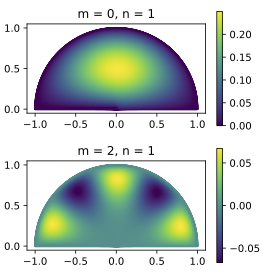
\includegraphics[width=\linewidth]{../graphs/base_functions copy.png}
  \caption{Examples of trial functions} \label{fig:a}
  \end{subfigure}
  \hspace*{\fill}
  \begin{subfigure}{0.5\textwidth}
  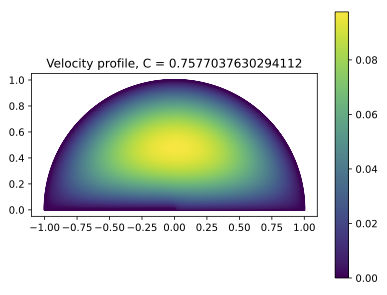
\includegraphics[width=\linewidth]{../graphs/velocity_field copy.png}
  \caption{Velocity profile.} \label{fig:b}
  \end{subfigure}
  \medskip
  \begin{subfigure}{0.5\textwidth}
  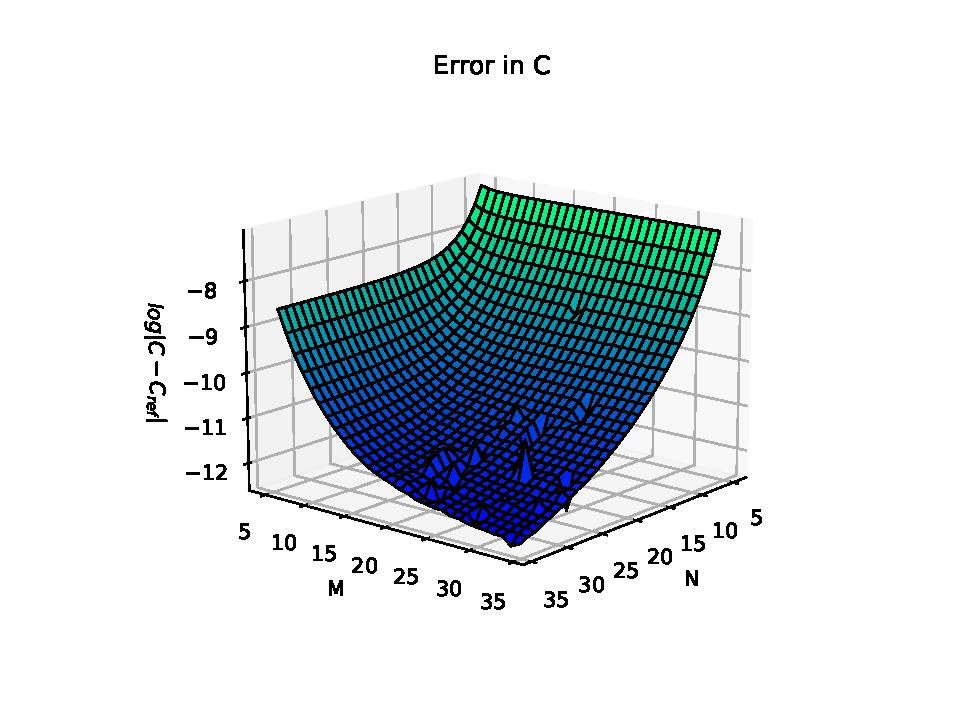
\includegraphics[width=\linewidth]{../graphs/error_in_c.pdf}
  \caption{Error in $C$ with respect to $N$ and $M$.} \label{fig:c}
  \end{subfigure}
  \hspace*{\fill}
  \begin{subfigure}{0.5\textwidth}
  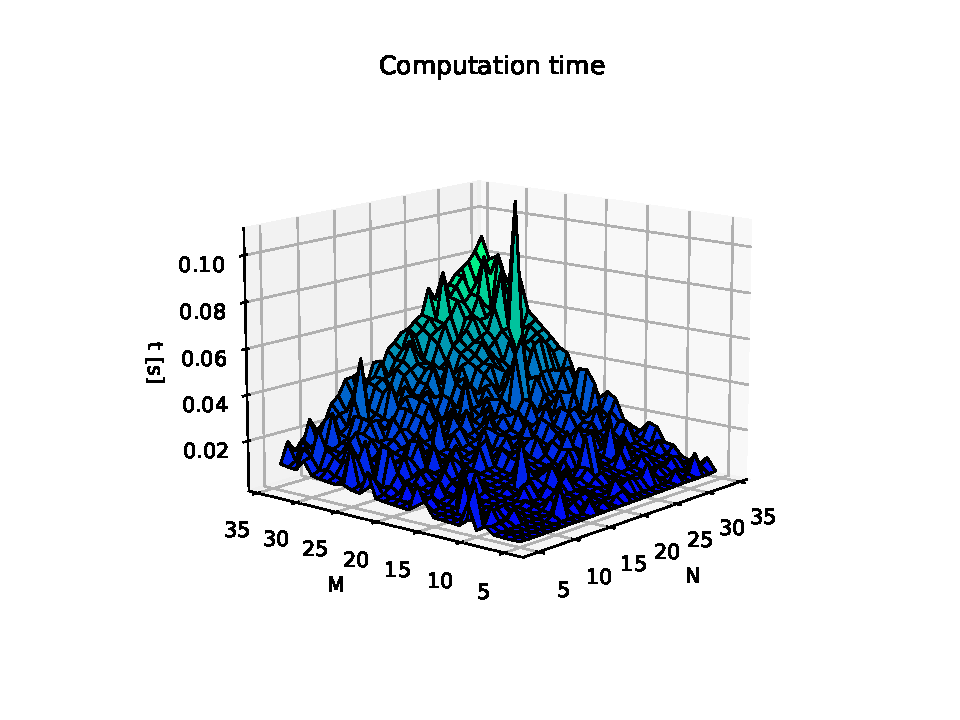
\includegraphics[width=\linewidth]{../graphs/time.pdf}
  \caption{Computation time with respect to $N$ and $M$.} \label{fig:d}
  \end{subfigure} 
  \caption{Analysis of the fluid flow solution.} \label{fig:1}
\end{figure}

To best measure the accuracy of the solution compared to factors like $N$ and $M$, we will use the constant $C$. As a reference $C_{ref}$ I chose the value computed at $N = 150$. This approach is not the best for evaluating the absolute accuracy, as some systemic error could shift all the values in one direction of the other. Such evaluation method is mostly suited for determining relative error. I ruled out the presence of a systematic error by comparing my solution with my peers. A better solution to that would be to solve the problem with Mathematica. Figure 1c presents the error in $C$ compared to $N$ and $M$, where we can observe that we quickly reach the reference value. Therefore $N = M = 30$ is sufficient for most purposes.

In the end let's look at the computation time. It's dependence on $N$ and $M$ is given in Figure 1d. We can conclude that for reaching a very accurate solution we don't require a lot of time. Timing complexity could also be improved, by using algorithms for solving band matrices.

\section{Hyperbolic wave equation}

The second problem we will be solving is the hyperbolic wave equation in one dimension
\begin{equation*}
  \frac{\partial u}{\partial t} - \frac{\partial u}{\partial \xi} = 0
\end{equation*}
for $\xi \in [0,2\pi]$ with periodic boundary conditions. The initial state is $u(\xi,0)=\sin(\pi\cos \xi)$. The analytical solution to this problem is $u(\xi,t)=\sin(\pi\cos(\xi+t))$. As with the previous problem we have to define a trial function. In this case the most obvious choice are waves $\Psi_j(\xi) = \frac{1}{\sqrt{2\pi}} \mathrm{e}^{\mathrm{i}j\xi}$ which are also orthogonal to each other. This simplifies our problem into a system of coupled differential equations for coefficients $a_k(t)$
\begin{equation*}
  \frac{da_k}{dt} - \mathrm{i}ka_k = 0 \>, \qquad
  k = -N/2, \dots, N/2 \>, \quad 
  a_k(0) = \int_0^{2\pi} u(\xi,0) \Psi^*_k(\xi) \dd \xi \>.
\end{equation*}

The solution to our problem is presented in Figure 2a and 2b, viewed from the top and from the side. Both of these were evaluated at $N = 150$. Such high value was chosen as the computation is very fast.

Figure 2c compared the numerical to the analytical solution. Some patterns can be observed from the graphs, but in general we see that the error is at around $10^{-14}$. This result also proves that there isn't any systematic error associated with this method. 

I also compared the coefficients $a_j(0)$ with the coefficients of the analytical solution, $a_k(t)=\sin\left(\frac{k\pi}{ 2}\right)\,J_k(\pi)\,\mathrm{e}^{\mathrm{i}kt}$. The absolute error is presented in Figure 2d, where we quickly ($j > 20$) reach the numerical limit.

\begin{figure}[hbtp]
  \begin{center}
  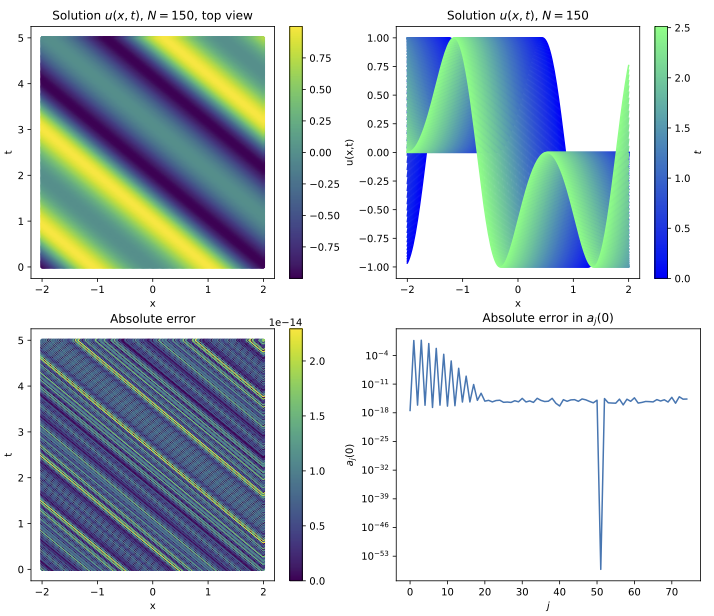
\includegraphics[width=13cm]{../graphs/dodatna_solution2 copy.png}
  \end{center}
  \vspace*{-7mm}
  \caption{Analysis of the hyperbolic wave equation solution.}
\end{figure}

\end{document}